\chapter{Project development}

To confirm the validity, both in terms of correctness and performance, of our algorithms we implemented all the procedures previously illustrated. 
The most important parts of the code can be found in the appendix of this thesis.

\section{Implementation choices and steps}

The algorithms have been implemented using the C++ programming language, 
as it provides good performance in practice and a lot of well implemented data structures in the Standard Template Library.\medskip

We have first implemented the $\textsc{brute}$ algorithm as it was the simpler and give us the correct answers, then we have implemented the three algorithms $\textsc{f-cont}$, $\textsc{f-samp}$, $\textsc{base}$ and check if some practical test gives us some reasonable values.
After making sure that all correctly works, we pass to parallelize them.\medskip

The parallelization has been implemented using the OpenMP API~\cite{openmp}, which defines a simple and flexible interface for developing parallel applications, in particular, we use it to manage the parallel for-loops and the critical sections.\medskip

To make the tests repeatable we used random generators with fixed seed, the subgraphs $A$ and $B$ were generated in three different ways: two random and independent subsets of $V$, two connected components (generated by choosing two random nodes and then expanding them through a $\textsc{BFS}$), two ego-networks.\medskip

All the code was written in a modular and highly customizable way in order
to better test the various algorithms, in the results we explicitly show the parameter used to execute the tests.

\clearpage

\section{Tuning the parameters in practice}

The problem can be applied to a lot of context.
That is why it is very important to choose the right domains for the values of the $V, E, L, \Sigma, q$:
\begin{itemize}
	\item $V$ are out object we want to modeling.
	\item $E$ represent the set of interactions, two vertices are connected if exists a relation among them.
	\item $L$ and $\Sigma$ are the category that partition $V$, $|\Sigma|$ should not be too high or too low, note that if $|\Sigma| = 1$ the labeling is useless as $V$ is not really partitioned.
	\item $q$ should be low as $N^{<q}(u)$ could be a large portion of $G$, (e.g. in Facebook for $q \simeq 4$ we have $N^{<q}(u) \simeq G$)~\cite{Facebook}.
\end{itemize}

\section{Dataset}

For the experiments we use two different kinds of dataset, a small one so we can easily brute-force the real indices and compare the relative errors, and a big one in order to benchmark the performance of the different approaches on a real world complex network.

\paragraph*{NetInf} This graph represents the flow of information on the web among blogs and news websites. The graph was computed by the \textit{NetInf} approach, as part of the \textit{SNAP} project~\cite{netinf}, by tracking cascades of information diffusion to reconstruct ``who copies who'' relationships.

\begin{itemize}
	\item $V$ is the set of blog or news website, $|V| = 854$.
	\item $E$, each website is connected to those who frequently copy their content, $|E| = 3824$.
	\item $\Sigma$ is the set of ranking class of websites ($0$ top $4\%$, $1$ next $15\%$, $2$ next $30\%$, $3$ last $51\%$), $|\Sigma| = 4$.
	\item $L$, each website is labeled according to its importance, using Amazon's Alexa ranking~\cite{alexarank}.
\end{itemize}

\textsl{Considered query:} compute the similarity of two websites $a$ and $b$ or two sets of websites.

\paragraph*{IMDb} In this graph, taken from the \textit{Internet Movie Database}~\cite{imdb} we have:

\begin{itemize}
	\item $V$ is the set of all movies in \textit{IMDb},  $|V| = 1\,060\,209$.
	\item $E$, two movies are connected if their casts share at least one actor, $|E| = 288\,008\,472$.
	\item $\Sigma$ is the set of movies genre, $|\Sigma| = 36$.
	\item $L$, each movie is labeled with its principal genre.
\end{itemize}

\textsl{Considered query:} similarity of actors' ego-networks. Given two actors $a$ and $b$, let $A$ and $B$ be their ego-networks, i.e., the sets of nodes corresponding to movies in which respectively $a$ and $b$ starred, compute the similarity of $A$ and $B$.\medskip

The way we generate the $\textsc{IMDb}$ graph is an example of collaboration graph and is known in literature as Co-stardom network. 

Another famous example is the collaboration graph of mathematicians, where two mathematicians are connected if they have co-authored a paper. 
This collaboration graph is also known as Erdős collaboration graph~\cite{BATAGELJ2000173}, in honor of the famous mathematician Paul Erdős, in this graph is defined also the \textit{Erdős number} as the distance in term of collaboration between Paul Erdős and another person.

\section{Experimental results}

We describe the experimental evaluation for our approach. Our computing platform is a machine with Intel(R) Xeon(R) CPU E5-2620 v3 at 2.40GHz, 24 virtual cores, 128 Gb RAM, running Ubuntu Linux v.4.4.0-22-generic. Code written in C++17, compiled with g++ v.5.4.1 and OpenMP 4.5.\medskip

To better analyze the different approaches described, we take several kinds of experiment in each of them~\footnote{Unless otherwise stated, all the results are the average of $100$ identical experiments, in order to reduce the possible errors randomly caused by the machine.}, all times are expressed in milliseconds.\medskip

An important fact of which to take into account is that we make large use of parallelization, 
so all the running time scale (approximately) linearly on the number of CPU cores used.

\subsection*{Running time}

In this experiment we compare the different running time, of all the parts, from all algorithms. Note that this is an important experiments, as in the real application time is crucial factor.\medskip

First of all we test how much we can go up in \textsc{Brute-Force} with the value of $q$ and the sample size, as this is our bottleneck to analyze the relative errors for the approximated methods.\medskip 

\begin{table}[h]
	\centering
	\begin{tabular}{|c|c|c|c|}
		\hline
		\textsc{Dataset} & $q$ & $|A \cup B|$ & \textsc{Brute-Force} \\ \hline \hline
		\textsc{NetInf}  & $4$ & $100$        & $200$                \\ \hline
		\textsc{NetInf}  & $4$ & $200$        & $420$                \\ \hline
		\textsc{NetInf}  & $4$ & $500$        & $870$                \\ \hline \hline
		\textsc{NetInf}  & $5$ & $100$        & $1\,206$             \\ \hline
		\textsc{NetInf}  & $5$ & $200$        & $2\,736$             \\ \hline
		\textsc{NetInf}  & $5$ & $500$        & $6\,080$             \\ \hline \hline
		\textsc{NetInf}  & $6$ & $100$        & $22\,715$            \\ \hline
		\textsc{NetInf}  & $6$ & $200$        & $49\,828$            \\ \hline
		\textsc{NetInf}  & $6$ & $500$        & $104\,129$           \\ \hline
	\end{tabular}
\end{table}

As expected, we can see that the running time for the bruteforce approach is linear in the size of $|A \cup B|$ and exponential in the value of $q$.\medskip

The second bottleneck for our algorithms is the preprocessing time for the dynamic programming table of color-coding, so we test for both the dataset how can we go up with the value of $q$. Always remembering from initial assumptions that the value of $q$ should not be too high. 

\begin{table}[h]
	\centering
	\begin{tabular}{|c|c|c|}
		\hline
		\textsc{Dataset} & $q$  & \textsc{Color-Coding} \\ \hline \hline
		\textsc{NetInf}  & $7$  & $20$                  \\ \hline
		\textsc{NetInf}  & $9$  & $80$                  \\ \hline
		\textsc{NetInf}  & $11$ & $185$                 \\ \hline
		\textsc{NetInf}  & $13$ & $340$                 \\ \hline
		\textsc{NetInf}  & $15$ & $1\,433$              \\ \hline \hline
		\textsc{IMDb}    & $3$  & $48\,220$             \\ \hline
		\textsc{IMDb}    & $4$  & $105\,943$            \\ \hline
		\textsc{IMDb}    & $5$  & $241\,224$            \\ \hline
		\textsc{IMDb}    & $6$  & $557\,481$            \\ \hline
	\end{tabular}
\end{table}

We can observe that, even in \textsc{IMDb} dataset, the value of $q$ could go high as expected, always remaining under $10$ minutes of running time. \medskip

To better understand these values, the official \textsc{IMDb} statistic~\cite{imdbstat} told us that, out of $1\,837\,357$ actors analyzed, $1\,579\,193$ ($\sim86\%$) are distant $q=3$ from the actor \textit{Kevin Bacon} and $1\,795\,352$ ($\sim98\%$) are distant $q=6$.\medskip

Finally, we test the running time for the different approaches for different value of $q$ and number $R$ of $q$-paths sampled. 

\begin{table}[h]
	\centering
	\begin{tabular}{|c|c|c|c|c|c|c|c|}
		\hline
		\textsc{Dataset} & $q$ & $|A|$ & $|B|$ & $R$      & \textsc{F-Count} & \textsc{F-Sample} & \textsc{Base} \\ \hline \hline
		\textsc{NetInf}  & $3$ & $100$ & $100$ & $1\,000$ & $20$             & $4$               & $2$           \\ \hline
		\textsc{NetInf}  & $3$ & $100$ & $100$ & $5\,000$ & $60$             & $30$              & $15$          \\ \hline
		\textsc{NetInf}  & $5$ & $100$ & $100$ & $1\,000$ & $2\,682$         & $426$             & $3$           \\ \hline
		\textsc{NetInf}  & $5$ & $100$ & $100$ & $5\,000$ & $4\,767$         & $784$             & $20$          \\ \hline
		\textsc{NetInf}  & $7$ & $100$ & $100$ & $100$    & $5\,455$         & $4$               & $2$           \\ \hline
		\textsc{NetInf}  & $7$ & $100$ & $100$ & $200$    & $16\,634$        & $197$             & $2$           \\ \hline \hline
		\textsc{IMDb}    & $3$ & $10$  & $10$  & $100$    & $5\,035$         & $66$              & $1$           \\ \hline
		\textsc{IMDb}    & $4$ & $10$  & $10$  & $1000$   & $/$              & $2\,829$          & $14$          \\ \hline
		\textsc{IMDb}    & $5$ & $10$  & $10$  & $1000$   & $/$              & $4\,739$          & $20$          \\ \hline
		\textsc{IMDb}    & $6$ & $10$  & $10$  & $1000$   & $/$              & $9\,783$          & $36$          \\ \hline
	\end{tabular}
\end{table}

The running time of \base is always extremely low, 
unlike \fcount that, as we already anticipated, is not suitable for sampling to many $q$-paths .
Instead the running time \fsamp results affordable for all the instance. 

This is because both the \fsamp and \base have a complexity of $O(rq)$ while 
\fcount, that analyze the $q$-paths inside $A \cup N^{<q}(A)$ and $B \cup N^{<q}(B)$, could possibly traverse all the graph.

\subsection*{Relative error and variance}

In this experiment we will compare, for increasing value of $R$, how accurate and stable are the different algorithms (using the $\textsc{NetInfo}$ dataset).\medskip

The accuracy is calculated with the average of the relative error between the exact solution of $\textsc{brute}$ and the analyzed algorithm \fcount, \fsamp or \base, instead the stability is calculated as the variance of the results $100$ experiments.

\begin{table}[h]
	\centering
	\begin{tabular}{|c|c|c|c|c|c|c|c|}
		\hline
		$q$ & $|A|$ & $|B|$ & $R$      & $\epsilon_{BC}$ & $\textsc{VAR}_{BC}$ & $\epsilon_{FJ}$ & $\textsc{VAR}_{FJ}$ \\ \hline \hline
		$3$ & $100$ & $100$ & $10$     & $0.02617187$    & $0.00082663$        & $0.02431909$    & $0.000190515$       \\ \hline
		$3$ & $100$ & $100$ & $100$    & $0.02258048$    & $0.00003059$        & $0.02324100$    & $0.000007628$       \\ \hline
		$3$ & $100$ & $100$ & $1\,000$ & $0.03952676$    & $0.00000070$        & $0.04030510$    & $0.000000132$       \\ \hline \hline
		$4$ & $100$ & $100$ & $10$     & $0.03828302$    & $0.00127922$        & $0.03703453$    & $0.000341645$       \\ \hline
		$4$ & $100$ & $100$ & $100$    & $0.01232044$    & $0.00005457$        & $0.00939392$    & $0.000016680$       \\ \hline
		$4$ & $100$ & $100$ & $1\,000$ & $0.01810665$    & $0.00000240$        & $0.02072427$    & $0.000000750$       \\ \hline \hline
		$5$ & $100$ & $100$ & $10$     & $0.04120389$    & $0.00199562$        & $0.04766193$    & $0.000590912$       \\ \hline
		$5$ & $100$ & $100$ & $100$    & $0.01418216$    & $0.00021613$        & $0.01550921$    & $0.000045352$       \\ \hline
		$5$ & $100$ & $100$ & $1\,000$ & $0.02144092$    & $0.00000647$        & $0.02015720$    & $0.000018239$       \\ \hline
		
	\end{tabular}
	\caption{Relative error and variance of the \fcount approach}	
\end{table}

\begin{table}[h]
	\centering
	\begin{tabular}{|c|c|c|c|c|c|c|c|}
		\hline
		$q$ & $|A|$ & $|B|$ & $R$      & $\epsilon_{BC}$ & $\textsc{VAR}_{BC}$ & $\epsilon_{FJ}$ & $\textsc{VAR}_{FJ}$ \\ \hline \hline
		$3$ & $100$ & $100$ & $10$     & $0.53290243$    & $0.02463258$        & $0.64549929$    & $0.01098586$        \\ \hline
		$3$ & $100$ & $100$ & $100$    & $0.26679417$    & $0.00291718$        & $0.35897713$    & $0.00141635$        \\ \hline
		$3$ & $100$ & $100$ & $1\,000$ & $0.05437719$    & $0.00023471$        & $0.12111130$    & $0.00015040$        \\ \hline \hline
		$4$ & $100$ & $100$ & $10$     & $0.56332930$    & $0.03922519$        & $0.71466000$    & $0.01504646$        \\ \hline
		$4$ & $100$ & $100$ & $100$    & $0.42694364$    & $0.00315346$        & $0.58182255$    & $0.00148827$        \\ \hline
		$4$ & $100$ & $100$ & $1\,000$ & $0.17956068$    & $0.00028600$        & $0.26846896$    & $0.00016087$        \\ \hline \hline
		$5$ & $100$ & $100$ & $10$     & $0.56603667$    & $0.03097334$        & $0.72217070$    & $0.01117576$        \\ \hline
		$5$ & $100$ & $100$ & $100$    & $0.60814392$    & $0.00324602$        & $0.73568322$    & $0.00098974$        \\ \hline
		$5$ & $100$ & $100$ & $1\,000$ & $0.37832023$    & $0.00030943$        & $0.49424173$    & $0.00010248$        \\ \hline
	\end{tabular}
	\caption{Relative error and variance of the \fsamp approach}	
\end{table}

\begin{table}[h]
	\centering
	\begin{tabular}{|c|c|c|c|c|c|c|c|}
		\hline
		$q$ & $|A|$ & $|B|$ & $R$      & $\epsilon_{BC}$ & $\textsc{VAR}_{BC}$ & $\epsilon_{FJ}$ & $\textsc{VAR}_{FJ}$ \\ \hline \hline
		$3$ & $100$ & $100$ & $10$     & $0.79011542$    & $0.023361286$       & $0.83428722$    & $0.00522323$        \\ \hline
		$3$ & $100$ & $100$ & $100$    & $0.38049732$    & $0.003518397$       & $0.40706656$    & $0.00123490$        \\ \hline
		$3$ & $100$ & $100$ & $1\,000$ & $0.10418507$    & $0.000494349$       & $0.10331303$    & $0.00011619$        \\ \hline \hline
		$4$ & $100$ & $100$ & $10$     & $0.89923793$    & $0.013469196$       & $0.90575658$    & $0.00365555$        \\ \hline
		$4$ & $100$ & $100$ & $100$    & $0.64715221$    & $0.004050390$       & $0.65129934$    & $0.00117385$        \\ \hline
		$4$ & $100$ & $100$ & $1\,000$ & $0.23606907$    & $0.000409090$       & $0.24419065$    & $0.00008983$        \\ \hline \hline
		$5$ & $100$ & $100$ & $10$     & $0.91908669$    & $0.009465890$       & $0.95246880$    & $0.00215748$        \\ \hline
		$5$ & $100$ & $100$ & $100$    & $0.82803890$    & $0.001517523$       & $0.83137675$    & $0.00062314$        \\ \hline
		$5$ & $100$ & $100$ & $1\,000$ & $0.44637460$    & $0.000352671$       & $0.46965620$    & $0.00004772$        \\ \hline
	\end{tabular}
	\caption{Relative error and variance of the \base approach}	
\end{table}

\clearpage

From the three previously tables we can clearly see that \fcount provide the best approximation for both the indices, 
with high precision and extremely low variance even for $R=10$. 
The \fsamp approach has a lower relative error compared to \base, however the variance between the two approaches are nearly the same.\medskip

We further investigate the variance between \fsamp and \base, this time using $\textsc{IMDb}$ as dataset,
in order to study the stability in a real application.

\begin{table}[h]
	\centering
	\begin{tabular}{|c|c|c|c|c|c|c|c|}
		\cline{5-8}
		\multicolumn{4}{c|}{} & \multicolumn{2}{c|}{\fsamp} & \multicolumn{2}{c|}{\base}\\
		\hline
		$q$ & $|A|$ & $|B|$ & $R$      & $\textsc{VAR}_{BC}$ & $\textsc{VAR}_{FJ}$ & $\textsc{VAR}_{BC}$ & $\textsc{VAR}_{FJ}$ \\ \hline 
		$3$ & $100$ & $100$ & $1\,000$ & $0.00000971$        & $0.00001004$        & $0.00011746$        & $0.00019368$        \\ \hline
		$4$ & $100$ & $100$ & $1\,000$ & $0.00000114$        & $0.00000736$        & $0.00012097$        & $0.00002175$        \\ \hline
		$5$ & $100$ & $100$ & $1\,000$ & $0.00000594$        & $0.00000085$        & $0.00004424$        & $0.00000624$        \\ \hline
		$6$ & $100$ & $100$ & $1\,000$ & $0.00000109$        & $0.00000020$        & $0.00001050$        & $0.00000154$        \\ \hline
	\end{tabular}
	\caption{Variance of \fsamp and \base}	
\end{table}

Now we can see that, for both indices, the variance of \fsamp is one, or in some case two, orders of magnitude fewer compared to \base.

A last test, always comparing \fsamp and \base on $\textsc{IMDb}$, we show some real values of the two indices comparing the ego-networks of the famous comic duo Laurel and Hardy
($q=3$, $R=1\,000$, $|A| = 186$ and $|B| = 415$).

\begin{table}[h]
	\centering
	\begin{tabular}{l|l|l|l|l|}
		\cline{2-5}
		&\multicolumn{2}{c|}{\fsamp} & \multicolumn{2}{c|}{\base}\\
		\cline{2-5}
		& \multicolumn{1}{c|}{BC} & \multicolumn{1}{c|}{FJ} & \multicolumn{1}{c|}{BC} & \multicolumn{1}{c|}{FJ} \\
		\cline{2-5}
		& 0.928940                & 0.780303                & 0.821951                & 0.638258                \\
		& 0.934292                & 0.759470                & 0.730479                & 0.549242                \\
		& 0.929231                & 0.770833                & 0.764780                & 0.575758                \\
		& 0.945752                & 0.787879                & 0.829152                & 0.657197                \\
		& 0.933196                & 0.780303                & 0.758974                & 0.560606                \\
		& 0.950655                & 0.793561                & 0.800000                & 0.621212                \\
		& 0.941658                & 0.761364                & 0.759051                & 0.575758                \\
		& 0.934292                & 0.776515                & 0.801980                & 0.613636                \\
		& 0.933333                & 0.761364                & 0.799020                & 0.617424                \\
		& 0.931282                & 0.768939                & 0.766917                & 0.579545                \\
		\hline
		\multicolumn{1}{|c|}{Mean}     & 0.936167                & 0.774053                & 0.783230                & 0.598864                \\
		\multicolumn{1}{|c|}{Variance} & 0.000055                & 0.000136                & 0.001005                & 0.001265                \\
		\hline
	\end{tabular}
	\caption{Values of estimated BC and FJ setting $A$ and $B$ respectively the movie ego networks of Stan Laurel \& Oliver Hardy }
	\label{table:stanlio}
\end{table}
\subsection*{Fixed relative error}

In this experiment we set the relative error and compare, for each approach, how many paths $R$ we need to reach such relative error.\medskip

\begin{table}[h]
	\centering
	\begin{tabular}{|c|c|c|c|c|c|c|c|c|c|c|}
		\cline{3-11}
		\multicolumn{2}{c|}{} & \multicolumn{3}{c|}{\fcount} & \multicolumn{3}{c|}{\fsamp} & \multicolumn{3}{c|}{\base}\\
		\hline	
		$q$ & $\epsilon$ & R    & T    & VAR      & R         & T    & VAR      & R         & T   & VAR      \\ \hline
		$3$ & $0.20$     & $2$  & $1$  & $0.0725$ & $400$     & $1$  & $0.1194$ & $420$     & $1$ & $0.1150$ \\ \hline
		$3$ & $0.10$     & $3$  & $1$  & $0.0692$ & $1\,000$  & $1$  & $0.0601$ & $900$     & $1$ & $0.1338$ \\ \hline
		$3$ & $0.05$     & $4$  & $1$  & $0.0535$ & $3\,200$  & $1$  & $0.0273$ & $1\,500$  & $1$ & $0.1025$ \\ \hline
		\hline
		$4$ & $0.20$     & $3$  & $2$  & $0.0677$ & $1\,300$  & $1$  & $0.1194$ & $1\,300$  & $1$ & $0.2424$ \\ \hline
		$4$ & $0.10$     & $5$  & $4$  & $0.0532$ & $3\,200$  & $2$  & $0.0992$ & $2\,500$  & $2$ & $0.1806$ \\ \hline
		$4$ & $0.05$     & $10$ & $8$  & $0.0518$ & $8\,000$  & $4$  & $0.0612$ & $7\,900$  & $3$ & $0.1081$ \\ \hline
		\hline
		$5$ & $0.20$     & $5$  & $6$  & $0.0511$ & $5\,000$  & $4$  & $0.1678$ & $6\,000$  & $3$ & $0.2234$ \\ \hline
		$5$ & $0.10$     & $10$ & $18$ & $0.0370$ & $20\,000$ & $12$ & $0.0745$ & $30\,000$ & $8$ & $0.1234$ \\ \hline
		$5$ & $0.05$     & $20$ & $58$ & $0.0204$ & $80\,000$ & $30$ & $0.0376$ & $/$       & $/$ & $/$      \\ \hline
	\end{tabular}
	\caption{Dataset $\textsc{NetInf}$, $|A| = |B| = 100$}
\end{table}
\medskip

We can clearly see that \fcount performed very well, as it needs to sample a very little amount of $q$-paths to reach $\epsilon$.
Instead \fsamp and \base needs many more $q$-paths to reach the precision of \fcount, in particular note that in the last test \base cannot reach the preestablished relative error.\bigskip

\subsection*{Actors' ego-networks}

In order to show a real application easy to understand, we compare
some pairs of actors ego-networks (using \fcount algorithm with $q=3$ and $R=1\,000$):\medskip

\begin{table}[h]
	\centering
	\begin{tabular}{c|c|l|l}
		Actor/actress  & Actor/actress   & BC index & FJ index \\ 
		\hline
		Stan Laurel    & Oliver Hardy    & 0.936167 & 0.774053 \\
		Robert De Niro & Al Pacino       & 0.730935 & 0.231474 \\
		Woody Allen    & Meryl Streep    & 0.556071 & 0.222857 \\
		Meryl Streep   & Roberto Benigni & 0.482909 & 0.160181 \\
		%\hline
	\end{tabular}
\end{table}

\medskip

The values, respect the theory very faithfully for many reasons. \medskip

The Bray-Curtis index, as we already said, is always greater than the Frequency Jaccard and takes more into account the intersection:

the ego-networks of the famous comic duo Laurel and Hardy have a big intersection, this make the Bray-Curtis value very close to 1, however the Frequency-Jaccard is much smaller as Oliver Hardy starred in about $300$ movie without Stan Laurel.

One last observation about the couple Meryl Streep and Roberto Benigni: we have a big difference between the Bray-Curtis and the Frequency Jaccard, this can be due from the fact they are both famous actors (both won the Oscar Prize) who starred with a lot of other famous actors but they haven't starred together.

\subsection*{Parallelization efficiency}

As a last test, we show the parallelization efficiency in the computational time of the color coding table for different numbers of cores used.

\begin{table}[h]
	\centering
	\begin{tabular}{|c|c|c|c|c|c|}
		\cline{3-6}
		\multicolumn{2}{c}{} & \multicolumn{4}{|c|}{ Core } \\ 
		\hline
		Dataset           & $q$  & $24$       & $12$       & $6$        & $3$        \\  \hline \hline
		$\textsc{NetInf}$ & $11$ & $185$      & $199$      & $220$      & $358$      \\  \hline
		$\textsc{NetInf}$ & $13$ & $340$      & $503$      & $948$      & $1753$     \\  \hline
		$\textsc{NetInf}$ & $15$ & $1\,433$   & $2\,235$   & $4\,296$   & $7\,654$   \\  \hline \hline
		$\textsc{IMDb}$   & $3$  & $48\,220$  & $83\,271$  & $139\,107$ & $224\,815$ \\  \hline
		$\textsc{IMDb}$   & $4$  & $105\,943$ & $190\,719$ & $353\,856$ & $684\,342$ \\  \hline
		
	\end{tabular}
\end{table}

In $\textsc{NetInf}$, as it is a small dataset, we see only a slight improvement, 
however in \textsc{IMDb} times (approximately) doubles as the number of cores used is halved.
We can see the times on \textsc{IMDb} in the following plot (logarithmic scale for time, linear scale for cores).\bigskip

\begin{minipage}[h]{0.9\textwidth}
 \centering
 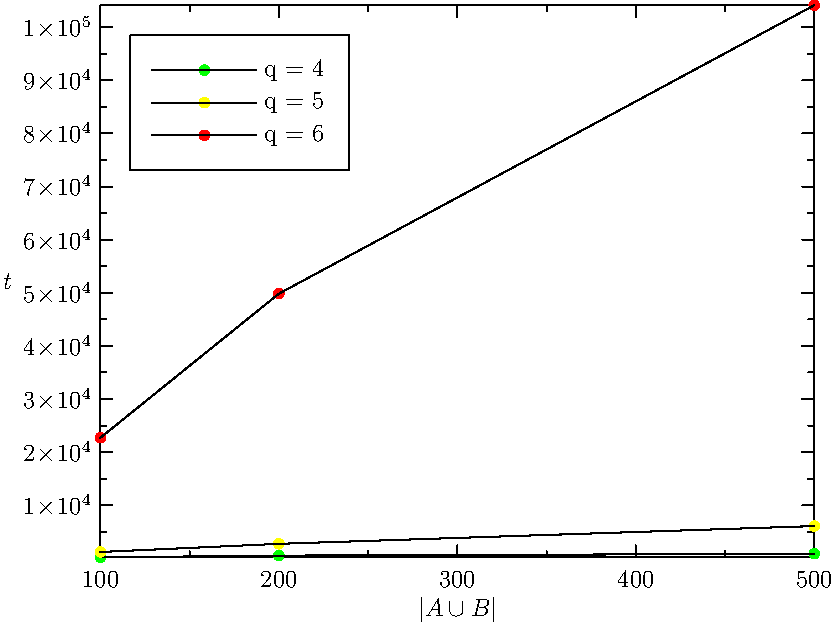
\includegraphics[width=0.9\textwidth]{figure/figure-4-1}
\end{minipage}

\clearpage